\documentclass[acmsmall,nonacm,screen]{acmart}
\usepackage{tikz}
\usepackage{color}
\usepackage{pgfplots}
\usepackage{amsmath}
\usepgfplotslibrary{groupplots,dateplot}
\usetikzlibrary{patterns,shapes.arrows}
\pgfplotsset{compat=newest}

\begin{document}

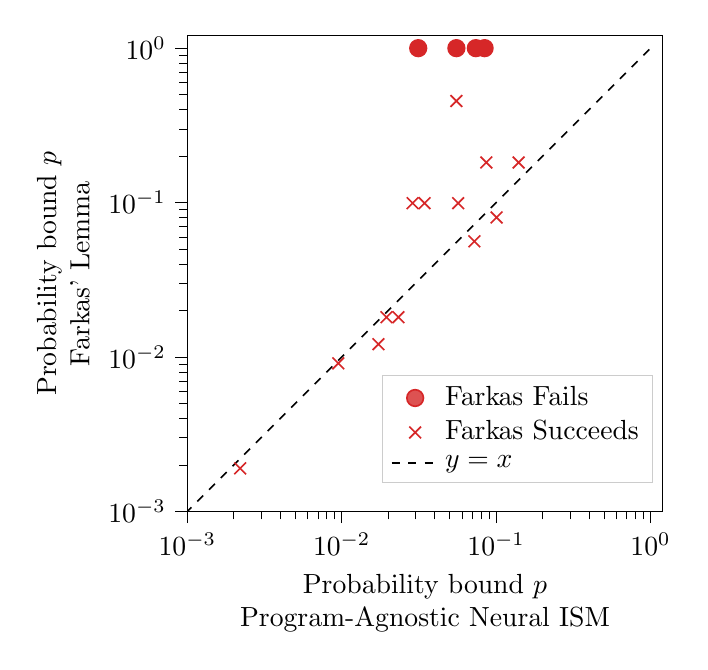
\begin{tikzpicture}

\definecolor{crimson2143940}{RGB}{214,39,40}
\definecolor{darkgray176}{RGB}{176,176,176}
\definecolor{lightgray204}{RGB}{204,204,204}

\begin{axis}[
legend cell align={left},
legend style={
  fill opacity=0.8,
  draw opacity=1,
  text opacity=1,
  at={(0.98,0.06)},
  anchor=south east,
  draw=lightgray204
},
log basis x={10},
log basis y={10},
tick align=outside,
tick pos=left,
x grid style={darkgray176},
xlabel style={align=center},
xlabel={Probability bound $p$\\Program-Agnostic Neural ISM},
xmin=0.001, xmax=1.2,
xmode=log,
xtick style={color=black},
y grid style={darkgray176},
ylabel style={align=center},
ylabel={Probability bound $p$\\Farkas' Lemma},
ymin=0.001, ymax=1.2,
ymode=log,
ytick style={color=black},
width=3in,
height=3in
]
\addplot [semithick, crimson2143940, mark=*, mark size=3, mark options={solid}, only marks]
table {%
0.0842 1
0.0739 1
0.0553 1
0.0313 1
};
\addlegendentry{Farkas Fails}
\addplot [semithick, crimson2143940, mark=x, mark size=3, mark options={solid}, only marks]
table {%
0.0288 0.0991
0.0344 0.0991
0.0568 0.0991
0.0864 0.1819
0.1399 0.1819
0.0095 0.0091
0.0195 0.0181
0.0233 0.0181
0.0022 0.0019
0.1007 0.0801
0.0723 0.0561
0.0173 0.0121
0.0553 0.4546
};
\addlegendentry{Farkas Succeeds}
\addplot [semithick, black, dashed]
table {%
0.0001 0.0001
1 1
};
\addlegendentry{$y=x$}
\end{axis}

\end{tikzpicture}

\end{document}